\subsubsection{Distribution of nodes: Graph coloring}
In order to implement a parallel asynchronous version of Tutte algorithm, it is necessary to separate graph nodes into different sets. The objectif is to extract an independance between nodes. In fact, each node have to move while maintaining neighbors positions. Thus, the independance must be between node and his neighbors. This problem is similar to the famous problem of graph colorating.
\paragraph*{}
The objectif of the modified Tutte algorithm is to handle graph of thousands nodes. To separate such a number of nodes, it is more performant to use a heuristic of the algorithm of graph coloring.\\
The greedy algorithm is a simple and good solution to separate nodes into sets fastly and effictively.
\paragraph*{}
The algorithm used in this project is :
\begin{verbatim}
G={V,E}
Y = V
color = 0
While Y is not empty
   Z = Y
   While Z is not empty
      Choose a node v from Z
      Colorate v with color
      Y = Y - v
      Z = Z - v - {neighbors of v}
   End while
   color ++
End while
\end{verbatim}
\subsubsection{Applying Tutte algorithm to sets}
Once a sets of nodes is obteined, it is possible to apply a parallel Tutte algorithm. The question is how to parallelize it on sets of nodes. The natural idea is to attribute one sets per thread :
\begin{figure}[!h]
\centering
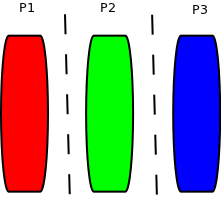
\includegraphics[scale=0.5]{img/distribution_verticale.png}
\caption{One set per thread}
\end{figure}
This distribution is far from being optimal. In fact, each thread have to lock neighbors node before moving it, wich introduce an importante critical section. In addition to being unfair, this distribution is limited by number of sets produced.\\

The best distribution for sets obteined by graph coloring is to execute $n$ threads on one set. Each thread move an number of nodes of the set without any critical section. This is because each node of the set is not the neighbor of all others nodes of the same set. Once the thread finish moving all his nodes of the set, he must wait for others threads (implemented by a barrier). After, the same processus is applyed on the next set.

\begin{figure}[!h]
\centering
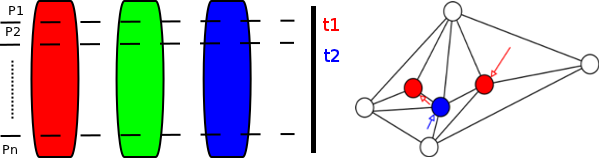
\includegraphics[scale=0.5]{img/distrib.png}
\caption{$n$ threads per set}
\end{figure}


Reference : Introduction to Algorithms (Cormen, Leiserson, Rivest, and Stein) 2001, Chapter 16 "Greedy Algorithms".
